\section{Auswertung}
\label{sec:Auswertung}
\paragraph{Bestimmung des Polarisationswinkels}
Der im Versuchsaufbau verwendete Polarisationsfilter soll so eingestellt werden, dass maximaler Kontrast 
gewährleistet ist. Dazu wird der Winkel gegen den Kontrast aufgetragen und der Kontrast kann mit nicht-linearer 
Ausgleichsrechnung bestimmt werden (vgl. Gleichung \eqref{eq:Kontrast2}). 
Die Ausgleichsrechnung wurde mit der der Gleichung 
\begin{equation*}
K(\theta) = \lvert a \cdot \sin(b \cdot \theta) +c \rvert	
\end{equation*}
durchgeführt, daraus ergeben sich die Parameter $a = \SI{0.72(4)}{}$, $b = \SI{1.85(3)}{}$ und 
$c = \SI{-0.08(3)}{}$.
Damit kann dann der Winkel für den größten Kontrast bestimmt werden. Die 
Prozedur ist in der Abbildung \ref{fig:K} abgebildet. Die Werte dazu sind in der Tabelle \ref{tab:KP} 
dargestellt. Der Polarisationswinkel mit größt möglichem Kontrast 
wurde zu $\theta \approx \SI{48}{\degree}$ bestimmt.
\begin{figure}
  \centering
  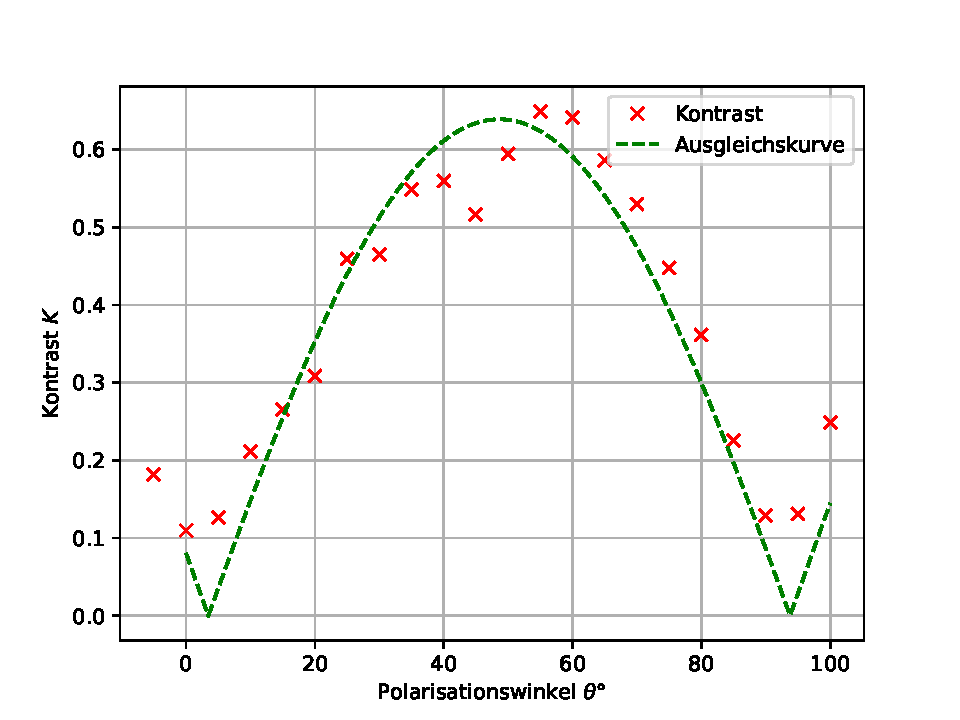
\includegraphics[height = 10cm]{plots/Kontrastfit.pdf}
  \caption{Kontrast aufgetragen gegen den Polarisationswinkel.}
  \label{fig:K}
\end{figure}
\begin{table}
 \centering
 \sisetup{round-mode = places , round-precision = 0,scientific-notation=fixed, fixed-exponent = 0}
 % \resizebox{\textwidth}{!}{%
 \begin{tabular}{S S[round-mode = places , round-precision = 2,scientific-notation=fixed, fixed-exponent = 0]}
   \toprule
    $\text{Plarisationswinkel} \; \theta / \si{\degree}$ &
    $\text{Kontrast} \; K $\\
   \midrule
	-5.000000000000000000e+00 & 1.816838995568685056e-01\\
	0.000000000000000000e+00 & 1.095538425601495225e-01\\
	5.000000000000000000e+00 & 1.261091691314869256e-01\\
	1.000000000000000000e+01 & 2.116923076923077351e-01\\
	1.500000000000000000e+01 & 2.649742823958852189e-01\\
	2.000000000000000000e+01 & 3.085736862900039790e-01\\
	2.500000000000000000e+01 & 4.594594594594594850e-01\\
	3.000000000000000000e+01 & 4.646237043713385417e-01\\
	3.500000000000000000e+01 & 5.483870967741935054e-01\\
	4.000000000000000000e+01 & 5.595334960672632141e-01\\
	4.500000000000000000e+01 & 5.163870967741935880e-01\\
	5.000000000000000000e+01 & 5.942499420357059137e-01\\
	5.500000000000000000e+01 & 6.487889273356401976e-01\\
	6.000000000000000000e+01 & 6.410256410256410797e-01\\
	6.500000000000000000e+01 & 5.861688431120103404e-01\\
	7.000000000000000000e+01 & 5.294117647058823595e-01\\
	7.500000000000000000e+01 & 4.477293508076805040e-01\\
	8.000000000000000000e+01 & 3.613016001075702865e-01\\
	8.500000000000000000e+01 & 2.258064516129032195e-01\\
	9.000000000000000000e+01 & 1.286857142857142644e-01\\
	9.500000000000000000e+01 & 1.309720842987972811e-01\\
	1.000000000000000000e+02 & 2.485212838165422322e-01\\
   \bottomrule
 \end{tabular}
 % }
 \caption{Kontrast in Abhängigkeit vom Polarisationswinkel}
 \label{tab:KP}
\end{table}

\FloatBarrier

\paragraph{Bestimmung des Brechungsindexes eines Glassplätchens}
Der Brechungsindex in Abhängigkeit von der Anzahl der Interferenzmaxima ist gegeben über
\begin{equation}
\delta M \approx \frac{2d}{\lambda_{vac}} \frac{n-1}{n} \cdot \theta_0 \cdot \delta \theta \;,
\label{eq:Mp}
\end{equation}
dabei bezeichnet $\delta M$ die Anzahl der Maxima, $d = \SI{1}{\milli\meter}$ 
die Dicke des Plätchens, $\lambda_{vac}=\SI{632.99}{\nano\meter}$ 
die Vakuumwellenlänge des Lasers, $\theta_0$ ist der Winkel zwischen 
den Plätchen und $\delta \theta$ die Winkeländerung. Das ist eine Korrektur die aufgrund der 
verwendeten Appartur auf der die Plätchen angebracht sind gemacht werden muss. 
Diese Gleichung ergibt sich aus der Entwicklung 
\begin{equation*}
\delta M = \left.\frac{\partial M}{\partial \theta} \right\rvert_{\theta = \theta_0 } \delta \theta
\end{equation*}
der Gleichung \eqref{eq:pM}, dabei ist $\theta_0 = \SI{10}{\degree}$.
Nun wird die Anzahl der Interferenzmaxima gegen die Winkeländerung aufgetragen und die Gleichung 
\eqref{eq:Mp} mit 
\begin{gather}
M = a \cdot \delta\theta \quad \text{mit} \quad a =\frac{2d \theta_0}{\lambda_{vac}} \frac{n-1}{n}
\label{eq:pfit} \\
\implies n = \frac{1}{1-\frac{\lambda_{vac} \cdot a}{2d \theta_0}} 
\label{eq:pbrech}
\end{gather}
verwendet, um über Ausgleichsrechnung den Parameter $a$ zu bestimmen. Das ist in der Abbildung 
\ref{fig:pfit} dargestellt. Die Daten dazu sind in der Tabelle \ref{tab:ptab} dargestellt.
Über die Gleichung \eqref{eq:pbrech} lässt sich dann der Brechungsindex bestimmen. Im Mittel 
ergibt sich ein Brechungsindex von $\bar{n} = \SI{1.0000000001068(7)}{}$. 
\begin{figure}
  \centering
  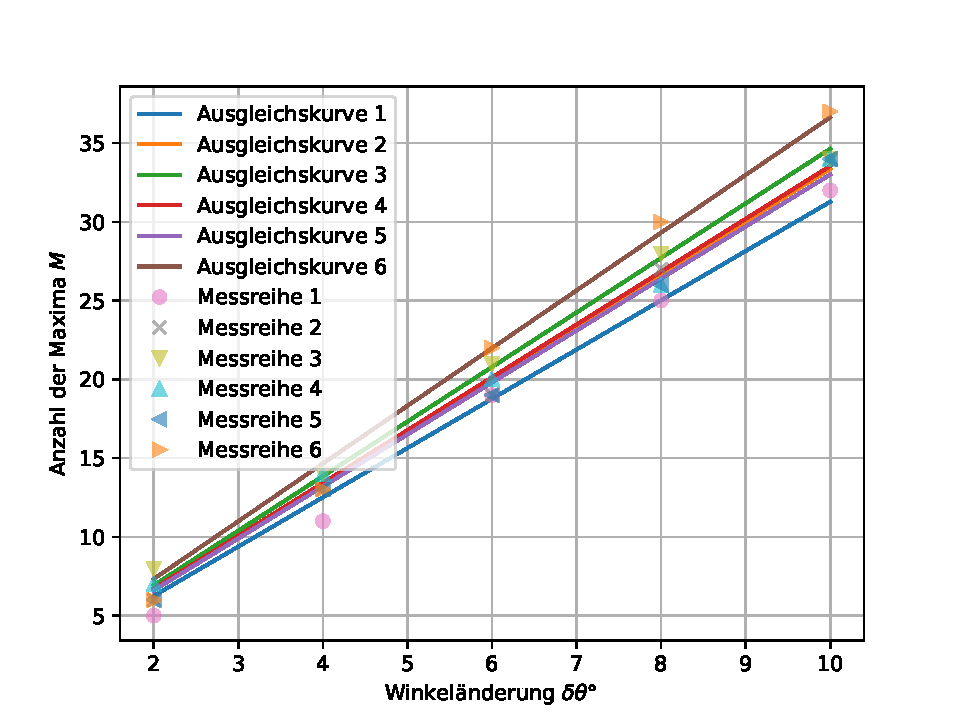
\includegraphics[height = 10cm]{plots/Plaettchenplot.pdf}
  \caption{Anzahl der Interferenzmaxima gegen die Winkeländerung aufgetragen für alle Messreihen.}
  \label{fig:pfit}
\end{figure}
\begin{table}
 \centering
 \sisetup{round-mode = places , round-precision = 0,scientific-notation=fixed, fixed-exponent = 0}
 % \resizebox{\textwidth}{!}{%
 \begin{tabular}{c S[round-mode = places , round-precision = 2,scientific-notation=fixed, fixed-exponent = 0]@{${}\pm{}$} S[round-mode = places , round-precision = 2,scientific-notation=fixed, fixed-exponent = 0] S[round-mode = places , round-precision = 12,scientific-notation=fixed, fixed-exponent = 0]@{${}\pm{}$} S[round-mode = places , round-precision = 0,scientific-notation=fixed, fixed-exponent = -12]}
   \toprule
	Messreihe & 
    \multicolumn{2}{c}{$\text{Parameter} \; a $} &
    \multicolumn{2}{c}{$\text{Brechungsindex} \; n $} \\
   \midrule
1 &  3.127272727277367270e+00 & 7.100226983043987639e-02 & 1.000000000098976605e+00 & 2.247186339443345078e-12\\ 
2 &  3.336363636497994278e+00 & 4.895604358213975771e-02 & 1.000000000105594200e+00 & 1.549434301680155337e-12\\ 
3 &  3.463636363641737326e+00 & 4.406981667204109415e-02 & 1.000000000109622311e+00 & 1.394787663067564263e-12\\ 
4 &  3.354545454592445353e+00 & 3.910147859407568649e-02 & 1.000000000106169740e+00 & 1.237542247025977809e-12\\ 
5 &  3.300000000005016254e+00 & 4.999999985240487221e-02 & 1.000000000104443343e+00 & 1.582474995659246426e-12\\ 
6 &  3.663636363642173155e+00 & 7.619570309656509277e-02 & 1.000000000115952359e+00 & 2.411555905713987907e-12\\ 
   \bottomrule
 \end{tabular}
 % }
 \caption{Ausgleichsparameter und die daraus berechneten Brechungsindizes im Überblick für jede Messreihe.}
 \label{tab:ptab}
\end{table}
\FloatBarrier

\paragraph{Bestimmung des Brechungsindexes von Luft}
Zur Bestimmung des Brechungsindexes bei Normalbedingungen von Luft wird die Anzahl der Interferenzmaxima 
in Abhängigkeit vom Druck gemessen. Die Anzahl der Interferenzmaxima wird dann mit der Gleichung 
\eqref{eq:lM} in einen Brechungsindex überführt. Über das Lorentz-Lorenz-Gesetz kann dann die 
Abhängigkeit von Druck und Brechungsindex untersucht werden, dazu wird die Nährung des Lorentz-Lorenz-Gesetz 
\eqref{eq:NLL} quadriert. 
Daraus ergibt sich folgende Gleichung und Abhängigkeit
\begin{equation}
n^2 = 1 + \frac{3Ap}{RT} \quad \rightarrow \quad n^2 = 1+ b \cdot p \; ,
\label{eq:brechl}
\end{equation}
damit kann über Ausgleichsrechnung der Parameter $b$ aus den Messwerten bestimmt werden. 
Die Prozedur ist in Abbildung \ref{fig:Lplot} dargestellt. 
Die dazugehörigen Daten sind in der Tabelle \ref{tab:ltab} dargestellt. 
Daraus ergibt sich dann im Mittel $ \bar{b} = \SI{5.80(5)e-09}{\per\Pa}$. 
Über 
\begin{gather}
b_V =  \frac{3A}{RT_V} \\
\frac{T_V}{T_N} \cdot b_V =\frac{3A}{RT_N} = b_N
\end{gather}
kann der Parameter $b_N$ bestimmt werden, dieser ist der Parameter für die Normalbedingungen 
($T_N = \SI{15}{\celsius}$) dabei bezeichnet $T_V = \SI{22,8}{\celsius}$ die Temperatur bei den die 
Messwerte aufgenommen wurden. 
Daraus folgt dann $ \bar{n_{N}} = 1 +  \bar{b_{N}} = \SI{1.000603(6)}{}$
\begin{figure}
  \centering
  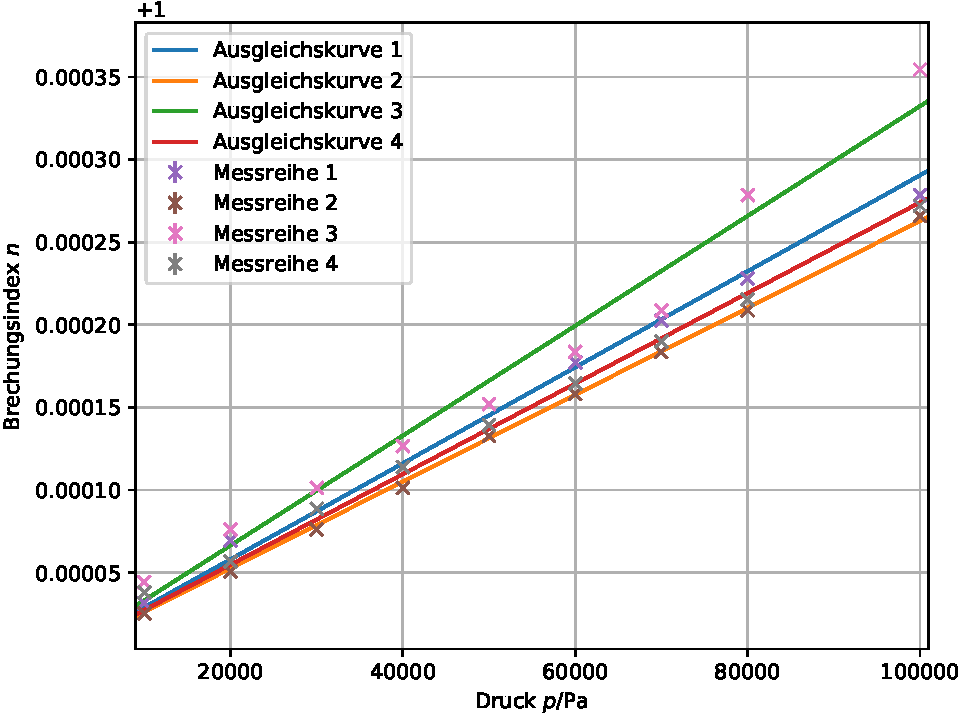
\includegraphics[height = 10cm]{plots/Luftplot.pdf}
  \caption{Brechungsindex von Luft in Abhängigkeit vom Druck.}
  \label{fig:Lplot}
\end{figure}

\begin{table}
 \centering
 \sisetup{round-mode = places , round-precision = 0,scientific-notation=fixed, fixed-exponent = 0}
 % \resizebox{\textwidth}{!}{%
 \begin{tabular}{c S[round-mode = places , round-precision = 2,scientific-notation=fixed, fixed-exponent = -9]@{${}\pm{}$} S[round-mode = places , round-precision = 0,scientific-notation=fixed, fixed-exponent = -11]}
   \toprule
	Messreihe &
    \multicolumn{2}{c}{$\text{Parameter} \; b / \si{\per\Pa} $}\\
   \midrule
1 &5.809969995581778485e-09 & 1.045533514818854323e-10\\ 
2 &5.256007599959811419e-09 & 2.621297613910566929e-11\\ 
3 &6.647253752729347500e-09 & 1.779406639991625090e-10\\ 
4 &5.480922540766930301e-09 & 5.797342151009091405e-11\\ 
   \bottomrule
 \end{tabular}
 % }
 \caption{Parameter aus den Ausgleichsrechnungen aus jeder Messreihe.}
 \label{tab:ltab}
\end{table}

